% interactcadsample.tex
% v1.03 - April 2017

\documentclass[]{interact}

\usepackage{epstopdf}% To incorporate .eps illustrations using PDFLaTeX, etc.
\usepackage{subfigure}% Support for small, `sub' figures and tables
%\usepackage[nolists,tablesfirst]{endfloat}% To `separate' figures and tables from text if required

% \usepackage{graphicx}
\usepackage{diagbox}
\usepackage{multirow}
\usepackage{comment}
\usepackage{xcolor}

\newcolumntype{P}[1]{>{\centering\arraybackslash}m{#1}}

\usepackage{natbib}% Citation support using natbib.sty
\bibpunct[, ]{(}{)}{;}{a}{}{,}% Citation support using natbib.sty
\renewcommand\bibfont{\fontsize{10}{12}\selectfont}% Bibliography support using natbib.sty

\theoremstyle{plain}% Theorem-like structures provided by amsthm.sty
\newtheorem{theorem}{Theorem}[section]
\newtheorem{lemma}[theorem]{Lemma}
\newtheorem{corollary}[theorem]{Corollary}
\newtheorem{proposition}[theorem]{Proposition}

\theoremstyle{definition}
\newtheorem{definition}[theorem]{Definition}
\newtheorem{example}[theorem]{Example}

\theoremstyle{remark}
\newtheorem{remark}{Remark}
\newtheorem{notation}{Notation}

\begin{document}

\articletype{ARTICLE TEMPLATE}

\title{A Novel Optimization Framework For Optimal Sensor Deployment In Smart Buildings }

\author{
\name{Anshul Agarwal \textsuperscript{a}\thanks{CONTACT Anshul Agarwal Email: anshula@iitb.ac.in , a.anshul215@gmail.com } and Krithi Ramamritham\textsuperscript{a}}
\affil{\textsuperscript{a} Department of Computer Science and Engineering, Indian Institute of Technology (IIT) Bombay, India.}
}

\maketitle

\begin{abstract}
  Smart buildings are considered to be the new age buildings. They are expected to evolve continuously and provide intelligent solutions. This is achieved by sensing the different factors. The existing approaches overlook the problems associated with the deployment of a large number of sensors. However, this article presents a novel and holistic optimal sensor deployment method -- optimization framework for sensing different factors to make buildings smarter. It describes how intelligently using the existing information can lead to a reduction in sensors. The method is compared with the baseline approach which deploys sensors at all the locations where they should be sensed. This optimization framework has been compared with the baseline approach for an existing building. The results indicate that the newly developed optimization framework requires 72.92\% less sensors as compared to the baseline approach. This feature makes it an impressive proposition and results in much less in e-waste generation. 
\end{abstract}

\begin{keywords}
Smart Buildings; Sensor Deployment; Optimization Framework; Baseline Approach; Sensor Reduction;
\end{keywords}

\section{Introduction}



Internet of Things (IoT) and Cyber-Physical Systems (CPS) are the two very commonly heard terms nowadays. Due to the advent of these technologies, buildings have evolved from being intelligent to becoming smarter. A smart building is expected to fulfill tasks like monitoring the health of appliances, provide thermal comfort to the users \citep{elsevier_hvac}, track occupants in the building, and optimize and reduce the wastage of energy \citep{karmakar}. However, fulfilling these tasks requires sensing of factors such as energy consumption, occupancy and type of appliances that are switched ON. Therefore, it is important to deploy sensors in the building to sense these factors of interest \citep{anshul_sensys_demo}. 
% (Agarwal et al. 2016a).
There exist various techniques for placement of sensors in the buildings to sense different factors \citep{bellala_electrons, meyn}. However, these techniques do not consider the issues related to the deployment of a large number of sensors, such as increased user inconvenience and capital cost of procuring, installing, maintaining and upgrading the sensors, disturbing the aesthetics of the building, incremental investment on storage and communication facilities for the sensors and threat to privacy \citep{hitchhiker_sensors,stankovic_iot}. The most worrying drawback of these techniques is the increased generation of e-waste. 
In 2016, the CEO of SoftBank Group Corporation estimated that there would be at least a trillion connected devices around the world in the next 20 years \citep{IntofTrash}. However, the existing techniques fail to provide effective solutions with sensor minimization as an important parameter.


In fact, rapid research in data mining, algorithms, and machine/deep learning approaches has led to efficient techniques for processing large amounts of sensor data. This encourages the approach of throwing sensors at the problem so that large amounts of data are generated and can be processed to provide smart applications and experience. 

The objective of this article is to provide an approach that reduces the number of sensors to be deployed to overcome the various issues related to the deployment of a large number of sensors in a smart building. The major contribution of this article is a novel and holistic approach to optimal sensor deployment in buildings to make it smarter by sensing the factors of interest. It uses soft sensing, which implies inferring a factor from other set of factors, as the primary tool to reduce the deployment of sensors; it defines how existing information can be intelligently used to infer the factors of interest, and thus reduce the number of sensors to be deployed. For instance, \cite{occupancy_wifi} demonstrated how occupancy can be inferred in the buildings using the Wi-Fi signal information. The effectiveness of this approach is tested on a real-world problem of sensor deployment in an existent building to make it smarter and demonstrate an impressive reduction in sensors.

\section{Literature Review}

% \textbf{?? to review refs ?? ??}
This article  presents (a) a holistic optimization framework for satisfying BMS requirements (b) seamless deployment of hard  and soft sensors and  
(c) utilizing a minimum number of sensors and deploying them at the right places in a building. A survey of the work done in these and related areas is presented in this section. 

Integration of Internet of Things (IoT) with buildings has led to buildings becoming smarter. 
One of the challenges in smart buildings is the storage and analysis of real-time sensor data \citep{zanella, building_smart}.  
\cite{iot_sb_bigdata} proposed a technique for the integration of big data analytics and IoT for effectively dealing with real-time building sensor data. 
\cite{iot_sb_challenges}  described a holistic framework for integrating smart home objects into a cloud-centric framework.
\cite{iot_sb_ems_opti}  discussed the various practical challenges faced by IoT in smart buildings.
\cite{iot_sb_prototype} proposed an IoT framework that used smartphone and cloud platforms for saving energy and improving the home network intelligence.
\cite{iot_sb_safir} proposed an ARM compliant security framework using IoT.
\cite{iot_sb_wsn} discussed how wellness of the home residents is monitored to determine if they are fine and extended this approach to the smart building environment. 

% \cite{weng} used different information to optimally control plug level loads and HVACs for saving energy of the building.
% \cite{magno} proposed a low cost, wireless, easy to install, adaptable, and smart LED lighting system to automatically adjust the intensity of light for saving energy.
% \cite{basu}  described a sensor-based intelligent lighting system for future grid-integrated buildings.
% A technique for optimizing energy usage and improving the thermal comfort of residents in smart buildings is discussed by \cite{schumann_ems_buildings}.
% \cite{yang}  proposed an approach for learning interaction between the residents and nest learning thermostats in the building to improve energy savings and user comfort.
% Data-driven system to estimate personal energy footprint in real-time has been discussed by \cite{wei}. 
% % Shwehdi et al. (2015) presented a case study on how HVACs affect building energy consumption.
% % Factors such as power supply and others that are important for user comfort are discussed by Au-Yong et al. (2019).
% \cite{sb_energy_occupancy_gul} presented a work that illustrates the relationship between occupancy and energy behavior of the building.
% A novel approach of using environmental and room sensors to control the installed HVACs is demonstrated by \cite{inverted_hvac}.
% Using the resident’s feedback to maintain a comfortable temperature inside the room has been investigated by \cite{sb_thermal_participation}.

% \hrulefill

Buildings play an important role in efficient functioning of electric grids. 
It is important for building to not impose higher loads on the electric grids, since they have other factors that bring in uncertainties like renewable energy sources, dispatchable resources and storage devices \citep{tf_pricing}.
Supplying electricity to remote areas requires optimal sizing of hybrid renewable energy systems (HRES) such that load requirements are satisfied with the high reliability and low cost \citep{tf_renewable}. 
To minimize the total energy and operating cost of the microgrid, an efficient algorithm based on particle swarm optimization is proposed by \cite{tf_swarm}.  


There exist multiple works that discuss inferring a factor from other sets of factors \citep{anshuleEnergy16, balaji}.   
Using virtual sensors to abstract hard sensors for programmatically specifying high-level requirements has been described by \cite{virtual_senors}.   
Using Wi-Fi signals to infer the occupancy status and information has been demonstrated by \cite{occupancy_wifi, softgreen}.
Occupancy prediction using CO2 based physical and statistical modeling has been investigated by \cite{elsevier_co2}. 
\cite{elsevier_occ_realtime}  proposed an adaptive probabilistic occupancy prediction model.
\cite{brown_fan}  discussed a low cost and non-intrusive method for sensor network deployment to combines information such as sound level, case temperature, CO2 and motion.
Using inference models like support vector regression and ensemble models to manage building power is discussed by \cite{tcps_bellala}.  
A network of sensors and cloud infrastructure can be used to monitor different behaviour inside homes as discussed by \cite{sensors_cloud_behaviour}. 
The work uses different soft sensing approaches to infer different behavioural patterns.
 \cite{tcps_virtualpowermeter} have proposed a virtual power meter, an example of a soft sensor, for online load tracking.  
\cite{tcps_solarcast} have proposed a soft sensor model called as SolarCast for predicting solar power for smart homes.  
\cite{sensors_caawd} have discussed a type of soft sensor {context-aware accurate	wellness determination (CAAWD)} for estimating the wellness of elderly people in homes. 
%Similarly, Tian et. al. \cite{sensors_accelerometer_2layer} have proposed a soft sensor model for human activity recognition using a wearable accelerometer sensor.
A review article  is presented by \cite{scs_ob} to discuss modeling of occupancy behaviour and its effect on building performance.
Learning about occupants and their sleep patterns to optimally operate HVACs has been described by \cite{lu}. 
These work utilize various soft sensing approaches to infer different behavioural patterns.
But these soft sensing approaches are not holistic since they aim to sense only one kind of factor.  
To understand the behaviour of the buildings, the factors such as energy  consumption, occupancy, appliance information and air quality are sensed individually in the existing literature.
% Inferring occupancy from power consumption has been discussed by \cite{brown_fan}.
% A framework called as Quiver has been proposed by \cite{koh2016quiver} for actuating HVAC systems to enable perturbations of the control system safely.  
The optimization framework proposed in this article emphasizes that factors should be monitored in conjunction with each other to reduce the number of sensors to be deployed and obtain a better view about the building functioning.
% But in this article, we justify and show that all of the different facets should be monitored, as per the node requirement, in conjunction with each other to get a better knowledge of the building, while reducing the number of sensors required. 

\cite{chang} proposes a solution to  achieving observability by optimally deploying sensors in nodes by formulating it as an optimization problem.
%Meyn et. al. \cite{meyn} have proposed a greedy approach to solve this problem.
Even though it reduces the number of sensors to be allocated, it does not present a holistic approach for sensing multiple factors at different granules of a building, unlike the optimization framework proposed in this article.
% they focus observability of facets at a particular granule, thus limiting the benefits accrued from observability.   Our approach, on the other hand, is aimed to sense multiple facets at all the granules of the building.
\cite{bellala_electrons, meyn} sense factors using only physical sensors and ignore the problems associated with deployment of large  number of sensors. 
\cite{anshuleEnergy16} proposed a technique for reducing the number of sensors for sensing building factors.
% Also, Cardell-Oliver \& Sarkar \cite{buildsense_tcs} present a greedy approach for using fewer sensors for sensing the factors of the building. 
% and keeping a check on the budget. 
%They also present  how using nearest hour of the day predictor works best in creating virtual sensors for their setup. Thus they discuss how to select soft sensors from the initial set of data and select a good mix of physical and soft sensors to perform fine grained sensing of the building. 
%Their semantics of soft sensors do not cover our more general scenarios, for example, inferring one facet from other facets, and thus their solution needs to be extended. 
%Further, only temperature and humidity data and sensors are considered.
But the solution, unlike the proposed approach of this article, does not provide solutions with optimal allocation of sensors.
Pre-deployment strategies with respect to sensors are discussed by \cite{max_info_min_comm}.
But it demands a prerequisite knowledge about the outdoor area statistics beforehand. 
\cite{smartmeter} proposed a a smartmeter allocation method to sense power consumption of building.
But it considers only smartmeter sensors,  and thus fail to provide a generic minimum sensor allocation strategy.

A popular approach to represent building metadata has been proposed by \cite{brick}.
It discusses an improved technique for preparing a uniform schema to represent building metadata. % for representing metadata in buildings 
%%has been deployed on at least six different buildings, and 
%can be the next standard to be adopted by the building applications worldwide. 
But this approach contains a drawback; it assumes that sensors are already deployed in an intelligent way, and thus, does not propose any efficient technique for allocating the sensors. % for satisfying building requirements.
Therefore, the optimization framework proposed in this article can be added as a layer of optimal sensor deployment technique in this framework, enhancing it to be more holistic and pragmatic .%, thus help since it contains a drawback of not intelligently placing the sensors for satisfying building requirements.



% ?? ?? Determining the nodes to place the sensors at -- so that full observability can be obtained -- is usually posed as a constrained optimization problem \cite{5740876} or by using a greedy algorithm\cite{5400442}.  Though these approaches reduce the number of sensors required to be installed,  they mainly target observation of a facet at a particular granule, which restricts  number of applications making use  or benefiting from observability.






% ?? ?? In this paper, we  propose different generic sensor placement strategies which can be used to place sensors to sense any facet under different scenarios. \cite{hp,5400442} Uses only hard sensors to sense facets, which requires tackling of all  problems related to hard sensor deployment. \cite{6197536} Uses soft sensors to sense only one facet. Thus, it can be seen that  previous approaches do not provide a  holistic framework that can achieve full observability on any type of building, while suggesting the type, necessary number and optimal placement of sensors.




The problem of sensing building factors with reduced sensors is similar to observing the electric grid using least number of Phasor Measurement Unit (PMU) sensors.
% optimal Phasor Measurement Units (PMU) in the electric grid is similar to the problem of optimal sensing of facets in the building.
% is akin to the problem of optimal Phasor Measurement Units (PMU) in the electric grid.  
PMUs sensors help to estimate the state of electric grid by measuring line parameters like voltage and current phasors \citep{pmu}, which leads to observability of the grid.  
The electric grid is represented as a graph, where the set of nodes represent buses (power generation centers or electric substations) of electric grids,
and the edges of the graph correspond to the transmission lines between the the buses. 
It is not desirable to install PMUs on all the nodes to observe state of the grid since they are expensive sensors \citep{ree_centeno}. 
Therefore, the goal is to deploy reduced number of PMU sensors in the electric grid.
Numerous work has been done on developing solutions for placing minimum PMUs in the grid to achieve observability \citep{pmu_review, taxonomy_pmu}.
%A taxonomy of PMU placement approaches has been discussed by Manousakis et. al. \cite{taxonomy_pmu}.
Optimal PMU placement for observing the grid is NP-Complete as proven by  \cite{gyllstrom}. 
%Brueni \& Heath \cite{brunei}, with an unrealistic assumption that all nodes are zero injection nodes. 
%This assumption is eliminated in the work by Gyllstrom et. al. \cite{gyllstrom} where both zero and non-zero injection node are considered, and the problem of optimal PMU placement for both type of nodes is proven to be NP-Complete. Hence they  present a heuristic (greedy) approach, with a polynomial running time,  to solve the problem with adequate accuracy. 
Formulating optimal PMU placement as an optimization problem is discussed by \cite{soman, abur, xu}. %Abur \& Magnago \cite{abur} and  Xu \& Abur \cite{xu}. 
%This work was extended and a general ILP formulation considering both zero and non-zero injection nodes has been proposed by Dua et. al. \cite{soman}. The work also considers the problem of  multi staging of PMUs and handling the PMU outage. 
Comparing this problem with the goal tackled in this article, the optimal PMU placement problem considers only a single type of sensor (PMU).
In addition, it primarily focuses on sensing only one factor, that is voltage, since current value is obtained using Ohm's Law and Kirchhoff's laws. 
Thus, this is a relatively simple problem where only one sensor and one factor is considered. 
On the other hand, the proposed optimization framework of this article provides a holistic solution which deals with sensing multiple factors using a set of heterogeneous type of sensors, while ensuring that a minimum number of sensors are deployed in the building.


% \cite{virtual_senors, balaji} have proposed techniques about using soft sensors for inferring facets from other set of facets.
% %Soft or virtual sensors are  used to abstract physical sensors and the operations performed on them \cite{virtual_senors}. 
% There exist many works that use soft sensor by exploiting contextual information like Wi-Fi probe requests, house structure, CO$_2$ information,  and other factors to infer occupancy information \cite{occupancy_wifi, tcps_schedule_infer, elsevier_occ_realtime, ss_occupancy_CO2}. 
%\cite{occupancy_wifi, sensors_occ_wifi, elsevier_occ_wifi, elsevier_occ_realtime, ss_occupancy_CO2}.
%and helps in reducing the number of physical sensors to sense occupancy. 
%The authors use occupancy profiling to identity areas where occupancy monitoring is not necessary and thus further reduce sensors. 
%Some examples of soft sensors and their usage are discussed in  \cite{balaji}.
% But all of these soft sensing approaches discussed,  aim to sense only one kind of factor.
%Tracking energy footprint of building residents helps to analyze the energy consumption pattern of the buildings \cite{tosn_footprint}.
%Using occupancy modeling to make building energy efficient has been discussed by Erickson et. al. \cite{tosn_erickson}.


%Some techniques (e.g.,\cite{vivek,anshul_buildsys_16}) only consider sensor minimization, and do not provide optimal solutions and also do not discuss about satisfying multiple requirements.

% Anshul et. al. \cite{anshul_buildsys_16} have proposed a heuristic algorithm that makes use of soft and hard sensors to reduce the number of sensors for sensing any kind of facet. But some of the drawbacks of this algorithm are: 
% %\noindent {\it Drawbacks of the heuristic algorithm }\\
% % Considers only sensor minimization; does not talk about other requirements like cost and error
% % Can the #sensor be further reduced? -- uses fewer #sensors, and not optimal #sensors
% % Different algorithms for satisfying different requirements
% % Does not consider the impact on the satisfaction of other requirements
% % Does not satisfy multiple requirements at the same time
% a) The heuristic algorithm considers only sensor minimization as the goal. But in real world, there may be other requirements that should be satisfied, like providing quality of service by minimizing error. 
% b) The algorithm reduces the number of sensors, but does not give an optimal number of sensors.
% c) In addition to satisfying single requirements, sometimes there is a need to satisfy multiple requirements simultaneously, like providing quality of service with minimum cost.
% Thus to overcome these drawbacks, the sensing framework has been proposed which provides a holistic approach of sensing facets while satisfying the BMS requirements.


%But this technique only reduces the number of sensors and does not provide an end to end solution of answering user queries by using minimum or optimal number of sensors.
%Optimally selecting the best sensor readings to increase the confidence in the answers to the sensor query for a high fidelity representation of real world phenomenon is presented in \cite{deshpande}.
%Authors in \cite{imprecise_data} discuss how to meaningfully answer the queries, where imprecision information is explicitly specified. 
%As far as we know, ours is the first approach to consider the hard and soft sensing capabilities to use optimal  number of hard sensors for achieving observability of different facets with specified attribute values  and thus answering the user queries using optimal number of sensors.

\begin{comment}
The optimal placement of Phasor Measurement Units (PMU), i.e., sensors for the grid, has been  studied previously. \cite{abur} \cite{xu} present an ILP optimization framework that solves the problem of optimal PMU placement, while achieving observability of all the nodes in the grid. \cite{soman} proposes multistaging of PMU placement using an ILP framework. 
% \cite{brueni} discusses PMU placement with zero injection nodes only, while \cite{kurose} includes non-zero injection nodes in the optimal PMU placement approach, both proving the respective problems to be NP-complete.
All these approaches consider only one type of sensor, i.e., PMU, and the two related facets, i.e., voltage and current.
Our problem is more complex due to the different observability requirements of facets at each node, and the heterogeneity of sensors and facets. 
Even if  techniques designed for PMUs can be applied to place smartmeters, because the laws governing current and voltage values can be used for both, in our problem we consider arbitrary sensors and building structures, which necessitate a different  and more general approach.
%Awareness about power consumption of buildings may encourage people to do the right things in order to conserve energy\cite{stern}. A lot of research has been done where energy consumption of  building is correlated to occupancy, number of appliances and temperature. There are various ways to observe each of the above stated factors. 
For example, various hard sensors like motion sensors and door sensors \cite{5779042}, pressure sensors \cite{1544421}, cameras, etc. are used to detect occupancy. Temperature of the building can be observed using temperature sensors and, the power consumption can be measured using smartmeters and clamp meters. These approaches, that are used to sense these facets, demand the installation of hard (physical) sensors and do not focus on reducing the number of sensors required.
% while ignoring the available contextual information 
The authors of \cite{6197536,6151374} demonstrate the usage of contextual or existing information to sense occupancy. But in general, these approaches fail to systematically capitalize on the readily available or other contextual information from other sources, which can be used to reduce the number of hard sensors required.
%%%%%%%%%%%%---
% With the increase in the number of smart buildings, the information that is available in these buildings is also increasing, and can be exploited to observe phenomena like occupancy, power consumption \cite{Palani}. In this article, we show how the existing information in the buildings can be used to observe many such phenomena thereby eliminating the need for a number of hard sensors.
%%%%%%%%%%%




Unlike \cite{Deshpande}, which takes a statistical approach to sense values, where the relationship between various facets is hidden, our article captures relationship between different facets and explicitly models them through a facet-sensor relationship graph. We also exploit the fact that one facet can serve as an input to another. These two techniques help to achieve observability of facets with a  minimum number of sensors. 
%%%%%%%%%%%%%%---
% This paper also demonstrates how a relationship exists between different facets and how value of one facet can be used to observe the value of another facet. This further reduces the number of hard sensors required to monitor.
%%%%%%%%%%%%%%%

%\vspace*{-2ex}




% Unlike \cite{hp,5400442} which uses only hard sensors and \cite{6197536} which uses soft sensors to sense only one facet, we fuse hard and soft sensors to observe multiple features. These steps leas to a large reduction in the costs of building and maintaining a BMS.



The solution proposed in this paper extends the discussion in \cite{observability_poster} and helps in systematically developing the framework to achieve full observability, using minimal infrastructure (hard sensors) and  using existing information and relation between facets and sensors. The observations can be used to implement (real-time) smart control decisions in different application scenarios, as was illustrated in the case of brownouts.

%In terms of future work, one question we will be seeking answers for is:\textit{In order to benefit from Observability, for how long does the BMS need to store the data of observed facets?}

% \hl{
% {\color{red}{
\cite{doukas} 
Presents a rule based approach for managing energy in a building. It proposes an integrated decision support model that attempts to guarantee a desirable thermal quality in all the rooms, while saving energy in the best possible way. The paper discusses how the decision agent will use the output from all the sensors to actuate appliances, thus providing the desired comfort in all the rooms while saving energy. 
\cite{Siano} Presents a survey on demand response (DR) potentials and  its benefits for the customers and smart grid. It presents how different sensors, communication systems and decision models help in effectively implementing DR in a smart grid. 
The approaches however do not emphasize on the need for strategic sensor placement in a building for managing energy.

\cite{Zhao} Presents a survey on the recently developed techniques to solve the problem of relating building energy consumption with the occupancy behaviour, appliance usage and ambient weather conditions. 
\cite{FREDERIKS} Discusses how key fundamentals from psychology and behavioural economics can be used to explain and change energy consumption behaviour of the customers. 
These techniques can be used in soft sensing techniques, which can further reduce the number of sensors required to manage energy in a building.


Observability is also important when there is a mix of renewable and non-renewable sources of energy. 
\cite{DINCER} Discussed different issues relating to renewable energy and sustainable development, conclusions of which are useful for energy scientists and policy makers. 
Observability helps in efficiently deciding which  amongst different renewable and non-renewable sources should be used to satisfy the energy consumption needs at a given time. 

In scenarios like blackout, batteries can help in reducing the discomfort of the users by providing some energy. \cite{battery} Presents an overview of different batteries that are used for large scale electricity storage.
\cite{Suganthi}  Presents a review of various energy demand forecasting models, which is required for proper allocation of the available resources for providing energy. 
As discussed earlier, observability can help in estimating the minimum energy consumption required during such scenarios, so that energy can be efficiently used from the batteries. 

\end{comment}



\begin{figure}[h]
  \centering
  \includegraphics[width=\linewidth]{{"images/linear sensor opti flow chart diagram"}.pdf}
  \caption{Block diagram summarizing the proposed approach}
  \label{f:block}
\end{figure}


\section{Methodology}

In this article, a new optimization framework has been developed for optimal sensor deployment. This optimization framework outputs the optimal number, type, and location of sensors such that required factors are sensed in the smart buildings. 


A block diagram to summarize the proposed optimization framework has been demonstrated in Figure \ref{f:block}.
The various inputs and symbols used in the framework are described in Table \ref{tab:var}.

\begin{table}[h]
\caption{Description of different symbols used in the optimization framework}
	\centering
	\begin{tabular}{p{0.15\textwidth}  p{0.8\textwidth}}
		\toprule
		\textbf{Input Variables} & \textbf{Description}
		\\ \midrule
		$\{L\}$                           & set of locations where factors are required to be sensed like rooms, levels and wings of the building
		\\ \hline
		$ \{K\} $                         & set of factors to be sensed in the building like occupancy and temperature
    \\ \hline
    $\{s^k\}$ & set of hard sensors to sense factors, where $s_i^k$ denotes sensor $s_i$ that senses factor k. For example, passive infrared sensors (PIR) and camera are used to sense occupancy
    \\ \hline
    $limit[s_i^k]$ & vector that denotes the limit on the number of sensors of type $s_i^k$ that can be deployed for sensing factor k. For example, \textit{limit(smartmeter) = 2} implies that a maximum of 2 smartmeters can be deployed to sense power
    \\ \hline
    $tosense[l,k]$ & a binary matrix, where 
    %  which denote whether factor k should be sensed at location l. The 
     a value of an element $e_{lk}$ is 1 if factor k should be sensed at location l; 0 otherwise
      % For example, tosense(HVAC,θ)=0 implies that occupancy should not be sensed in location HVAC room
    \\ \midrule
    \textbf{Output Variables} & \textbf{Description} 
    \\ \midrule
    $used(l,k,s_i^k)$  &  value of element is $1$ if sensor $s_i^k$ is allocated in location $l$ to sense factor $k$; $0$ otherwise 
    % number of  sensors of type $s_i^k$ allocated in location $l$  to sense factor $k$ 
    \\ \hline
    $sensed(l,k)$    & value of element is $1$ if factor $k$ is sensed in location $l$; $0$ otherwise
    % count of sensors that can sense facet $f$ on node $n$           
    \\ \bottomrule
	\end{tabular}
	\label{tab:var}
\end{table}

\subsection{Application Area}

For the application of optimization framework, a set of rooms of KReSIT building of the Computer Science and Engineering Department, IIT Mumbai (India) was selected. The building consists of one HVAC room and two levels. Each level consists of one small and one big room as shown in Figure \ref{f:app_topology}. Each big room was divided into two zones to sense different factors. A separate location for the HVAC room is denoted since it provides common cooling to all the rooms of the building and consumes a very high amount of energy. 


\begin{figure}[h]
  \centering
  \includegraphics[width=\linewidth]{{"images/application area topology"}.pdf}
  \caption{Representation of the application area building}
  \label{f:app_topology}
\end{figure}



\subsection{Optimization Framework}

It consists of an objective function and set of constraint functions which are described as follows.

\subsubsection{Objective Function}

Equation \eqref{e:obj} is used to specify the aim of deploying minimum number of sensors in the building to sense factors.
\begin{equation}
  \label{e:obj}
  minimize \sum_{l \in \{L\}} \sum_{k \in \{K\}} \sum_{s \in \{s^k\}}  used(l,k,s)
\end{equation}

\subsubsection{Constriant Functions}

\noindent $\diamond$ Sensing Requirement: this constraint is specified by Equation \eqref{e:sense_req} and ensures that the final optimal sensor allocation satisfies the sensing requirement required for the smart building.
\begin{equation}
  \label{e:sense_req}
  \forall l \in \{L\} \;\; \forall k \in \{K\} \quad sensed(l,k) = tosense(l,k)
\end{equation}



\noindent $\diamond$ Sensing Rules: A hard sensor denotes a physical sensor like smartmeter and temperature sensor. 
A soft sensor is defined as a model that infers a factor from the set of other available factors. An example of a soft sensor is inferring occupancy from available Wi-Fi signals \citep{occupancy_wifi}.  
Soft sensors can be used to reduce the number of hard sensors given the type of information available in a location.  
The following set of rules determine the sensing a factor $k$ at a location $l$ for a given allocation of sensor: % , the following sensing rules apply.

  \noindent Rule 1: If a hard sensor $s_i^k$ is allocated in location $l$, then the factor $k$ is sensible in location $l$. 
  This rule is denoted by Equation \eqref{e:1rule}.
\begin{equation}
  \label{e:1rule}
  \forall l \in \{L\} \;\; \forall k \in \{K\} \quad sensed(l,k) = 
  \sum_{s \in \{s^k\}}  used(l,k,s)  
  \end{equation}

  \noindent Rule 2: If a soft sensor, that infers factor $k$ from others factors $\{k_i\}$, is allocated in location $l$ and factors $\{k_i\}$ are sensible in location $l$, then the factor $k$ is sensible in location $l$.
  This rule is denoted by Equation \eqref{e:2rule}.
\begin{equation}
  \label{e:2rule}
  \forall l \in \{L\} \;\; \forall k \in \{K\} \quad sensed(l,k) = 
  \prod_{j \in \{k_i\}} sensed(l,j)
  \end{equation}

Combining Equations \eqref{e:1rule} and \eqref{e:2rule}, the constraint specifying the sensing rules is denoted by Equation \eqref{e:rules} as follows: 
\begin{equation}
  \label{e:rules}
  \forall l \in \{L\} \;\; \forall k \in \{K\} \quad sensed(l,k) = \max \left(
  \sum_{s \in \{s^k\}}  used(l,k,s) , 
  \prod_{j \in \{k_i\}} sensed(l,j)
  \right)
  \end{equation}

  \noindent $\diamond$ Sensing from sub-locations: A location may be composed of sub-locations or relatively small locations (Figure \ref{f:app_topology}). Let the sub-locations of a location l be represented by $\{subl^l\}$. Thus, this constraint states that if a factor k that is sensible in all the sub-locations of a location l, then the factor k is also sensable at location l. For example, consider a room that consists of two zones. 
  % To sense the temperature of a room,
  The temperature values of the room's sub-locations (zones) are aggregated using a function like average to represent the temperature of the room.
  This constraint is represented by Equation \eqref{e:sub_loc} as follows:
\begin{equation}
    \label{e:sub_loc}
    \forall l \in \{L\} \;\; \forall k \in \{K\} \quad sensed(l,k) = \max \left(
  \sum_{s \in \{s^k\}}  used(l,k,s) , 
  \prod_{sub \in \{subl_l\}} sensed(sub,k)
  \right)
  \end{equation}

  \noindent $\diamond$ Limiting the sensors: if $limit(s_i^k)$, which represents the maximum number of sensor $s_i$ sensing factor k that can be deployed, is provided as input, then this constraint ensures that the total number of sensors of the type $s_i^k$ deployed in the optimal sensor allocation does not exceed the provided limit.
  It is denoted by Equation \eqref{e:limit}.
\begin{equation}
  \label{e:limit}
    \forall k \in \{K\} \;\; \forall s \in \{s^k\} \quad \left(
      \sum_{l \in \{L\}} used(l,k,s)
    \right) \leq limit(s)
   \end{equation}


\section{Results And Discussion}

A smart building provides thermal comfort at optimum power consumption based on the occupancy using minimum number of sensors. It can be achieved by occupant detection and appliance automation. To fulfill these tasks, four primary factors need to be sensed: power consumption, number and type of ON appliances, occupancy and temperature of the rooms.

\subsection{Inputs used for optimal sensor allocation}

\begin{itemize}
  \item Set of Locations $\{L\}$: as represented in Figure \ref{f:app_topology}.
  \item Factors to Sense: power consumption, number and type of ON appliances, occupancy and temperature.
  \item Type of Sensors: used to sense the above factors as shown in Table \ref{t:sensors}.
\begin{table}[h]
\caption{List of sensors for sensing different factors}
	\centering
  \begin{tabular}{p{0.19\textwidth}|p{0.19\textwidth}|p{0.19\textwidth}|p{0.19\textwidth}|p{0.19\textwidth}}
    \toprule
    \textbf{Factors} & \textbf{Power} &  \textbf{Number of ON Appliances} &  \textbf{Occupancy} &  \textbf{Temperature}  
    % \backslashbox{\textbf{Sensor Type}}{\textbf{Factors}} & \textbf{Power} &  \textbf{Number of ON Appliances} &  \textbf{Occupancy} &  \textbf{Temperature}  
    \\ \midrule
    Hard Sensor	& Smartmeter &	Smart Switch &	PIR (passive infrared), Camera &	Temperature sensor
    \\ \hline
    Soft Sensor (infer from factors) &	Number of ON appliances &	Occupancy and Temperature &	- &	-
\\ \bottomrule
  \end{tabular}
  \label{t:sensors}
  \end{table}

\item Sensing Requirement: All the factors in all the locations, except HVAC room $(L^{H})$, should be sensed. 
This requirement is specified using Equation \eqref{e:req1} as follows:
\begin{equation}
  \label{e:req1}
  \forall l \in \{L \setminus L^{H} \} \;\; \forall k \in \{K\} \quad tosense(l,k) = 1
\end{equation}

For location HVAC room $L^{H}$, only power consumption should be sensed since the room is never occupied, and sensing other factors is not meaningful.
It is specified by Equation \eqref{e:req2} as follows:
\begin{equation}
  \label{e:req2}
  \begin{split}
    tosense(L^{H}, power) = 1 , \\
    \forall k \in \{K \setminus power \} \quad tosense(L^{H},k) = 0
  \end{split}
\end{equation}

\end{itemize}
  


\subsection{Output}

The optimization framework has been implemented in python library PuLP \citep{pulp} which is used for solving linear programs. When the various inputs (as discussed in the previous section) are given to the optimization framework, it implements the objective function Eq. (1) and constraint functions (Eq. (2) – (5)) to output the optimal sensor allocation for the application area, whose details are summarized in Table \ref{t:sensed_matrix} and Table \ref{t:used_matrix}.

\begin{table}
  \centering
  \caption{\textit{sensed} matrix denoting the factors that are sensable in different locations}
  \begin{tabular}{P{0.23\textwidth} P{0.09\textwidth} P{0.22\textwidth} P{0.14\textwidth} P{0.17\textwidth}}
    \toprule
    \textbf{Locations} &  \textbf{Power} &  \textbf{ON Appliances} &  \textbf{Occupancy} &  \textbf{Temperature}   
    \\ \midrule
    Building $B$	&	1	&	1	&	1	&	1	\\ \hline
    Level $L_1$	&	1	&	1	&	1	&	1	\\ \hline
    Level $L_2$	&	1	&	1	&	1	&	1	\\ \hline
    HVAC room	$H$ &	1	&	0	&	0	&	0	\\ \hline
    Small Room $SR_1$	&	1	&	1	&	1	&	1	\\ \hline
    Big Room $BR_1$	&	1	&	1	&	1	&	1	\\ \hline
    Zone $Z_{11}$	&	1	&	1	&	1	&	1	\\ \hline
    Zone $Z_{12}$	&	1	&	1	&	1	&	1	\\ \hline
    Small Room $SR_2$	&	1	&	1	&	1	&	1	\\ \hline
    Big Room $BR_2$	&	1	&	1	&	1	&	1	\\ \hline
    Zone $Z_{21}$	&	1	&	1	&	1	&	1	\\ \hline
    Zone $Z_{22}$	&	1	&	1	&	1	&	1	
\\ \bottomrule
    \end{tabular}
  \label{t:sensed_matrix}
\end{table}

\begin{table}
  \centering
  \caption{\textit{used} matrix denoting the details of sensor allocation}
  \begin{tabular}{P{0.16\textwidth}|P{0.15\textwidth}|P{0.19\textwidth}|P{0.06\textwidth}|P{0.1\textwidth}|P{0.17\textwidth}}
    \toprule
    \multirow{2}{*}{\textbf{Locations}} &
    \textbf{Power} & 
    \textbf{ON Appliances} & 
    \multicolumn{2}{c|}{\textbf{Occupancy}} &
    \textbf{Temperature} 
    \\ \cmidrule{2-6} 
    &
    \textbf{Smartmeter} &
    \textbf{Smart Switch} &
    \textbf{PIR} &
    \textbf{Camera} &
    \textbf{Temperature Sensor} 
    \\ \midrule
    Building $B$	&	0	&	0	&	0	&	0	&	0	\\ \hline
    Level $L_1$	&	0	&	0	&	0	&	0	&	0	\\ \hline
    Level $L_2$	&	0	&	0	&	0	&	0	&	0	\\ \hline
    HVAC room $H$	&	1	&	0	&	0	&	0	&	0	\\ \hline
    Small Room $SR_1$	&	0	&	0	&	1	&	0	&	1	\\ \hline
    Big Room $BR_1$	&	0	&	0	&	0	&	0	&	0	\\ \hline
    Zone $Z_{11}$	&	0	&	0	&	1	&	0	&	1	\\ \hline
    Zone $Z_{12}$	&	0	&	0	&	1	&	0	&	1	\\ \hline
    Small Room $SR_2$	&	0	&	0	&	1	&	0	&	1	\\ \hline
    Big Room $BR_2$	&	0	&	0	&	0	&	0	&	0	\\ \hline
    Zone $Z_{21}$	&	0	&	0	&	1	&	0	&	1	\\ \hline
    Zone $Z_{22}$	&	0	&	0	&	1	&	0	&	1	
    \\ \bottomrule
  \end{tabular}
  \label{t:used_matrix}
\end{table}


Observing the \textit{sensed} matrix (Table \ref{t:sensed_matrix}), it can be concluded that the sensing requirement of sensing all the factors in all the locations, except HVAC room where only power consumption should be sensed, is satisfied by the optimization framework. The details of optimal sensor allocation for satisfying the sensing requirements is denoted by \textit{used} matrix (Table \ref{t:used_matrix}) and are explained as follows. 

\begin{itemize}
  \item Since no soft sensor is available to sense temperature (Table \ref{t:sensors}), two hard sensors are used to sense the temperature in two small rooms (one for each room) and four sensors for big rooms (one for each zone). In big rooms, the temperature is sensable since temperature of the zones is sensed (Constraint C, Eq. (4)). Similarly, the temperature of levels and the building become sensable. Thus, a total of six temperature sensors are deployed.
  \item Occupancy is sensed either by placing Passive infrared (PIR) sensor or a camera in two small rooms (one for each room) and two big rooms (one for each zone). No soft sensor is used since occupancy cannot be inferred from the other factors in these locations. Using Constraint C Eq. (4), occupancy of big rooms, levels and the building becomes sensable. Therefore, a total of six PIR + camera sensors are deployed.
  \item Information of ON appliances can be inferred from occupancy and temperature using a soft sensor (Table \ref{t:sensors}). Since all the locations already sense temperature and occupancy, the number and type of ON appliances is sensed using the soft sensor (Constraint B, Eq. (3)). Therefore, no hard sensor is deployed to sense this factor.
  \item In the HVAC room, only one smartmeter is placed to sense power consumption since no other factor is sensed at this location. In all the remaining locations, power consumption is inferred from number and type of ON appliances information using a soft sensor (Constraint B, Eq. (3)).
\end{itemize}

Therefore, to sense the factors in all the locations of the building, only 13 sensors are required as tabulated in Table \ref{t:sensor_allo_opti}.

\begin{table}[h]
  \centering
  \caption{Sensor allocation for sensing the factors using the optimization framework}
  \begin{tabular}{|p{0.24\textwidth}|P{0.36\textwidth}|P{0.25\textwidth}|}
    \toprule 
  \textbf{Type of Hard Sensor} & \textbf{Location} & \textbf{Number of Sensors Allocated}
  \\ \midrule
  Temperature Sensor & $SR_1, Z_{11}, Z_{12}, SR_2, Z_{21}, Z_{22}$ & $6$
  \\ \hline
  PIR or Camera      & $SR_1, Z_{11}, Z_{12}, SR_2, Z_{21}, Z_{22}$ & $6$
  \\ \hline
   Smart Switch & -- & --
   \\ \hline
   Smartmeter & HVAC Room ($H$) &  $1$
   \\ \hline
   \multicolumn{2}{|l|}{\textbf{Total}} & \textbf{13}
   \\ \hline 
  \end{tabular}
  \label{t:sensor_allo_opti}
\end{table}


However, the effectiveness of the proposed optimization framework is compared with baseline approach method for sensor deployment at the same application area. The baseline approach consists of deploying appropriate sensors for all the factors in all the locations where they should be sensed. For example, to sense power, ON appliances, occupancy, and temperature at all the location of the building (Figure \ref{f:app_topology}), four sensors (one for each factor) is deployed in all the locations, leading to the deployment of 48 sensors as shown in Table \ref{t:sensor_allo_baseline}.


\begin{table}[h]
  \centering
  \caption{Sensor allocation for sensing the factors using the baseline approach}
  \begin{tabular}{|p{0.24\textwidth}|P{0.36\textwidth}|P{0.25\textwidth}|}
    \toprule 
  \textbf{Type of Hard Sensor} & \textbf{Location} & \textbf{Number of Sensors Allocated}
  \\ \midrule
  Temperature Sensor & $B,  L_1,  SR_1,  BR_1,  Z_{11},  Z_{12},$  $L_2,  SR_2,  BR_2,  Z_{21},  Z_{22},  H$ & $12$
  \\ \hline
  PIR or Camera  & $B,  L_1,  SR_1,  BR_1,  Z_{11},  Z_{12},$  $L_2,  SR_2,  BR_2,  Z_{21},  Z_{22},  H$ & $12$
  \\ \hline
   Smart Switch  & $B,  L_1,  SR_1,  BR_1,  Z_{11},  Z_{12},$  $L_2,  SR_2,  BR_2,  Z_{21},  Z_{22},  H$ & $12$
   \\ \hline
   Smartmeter  & $B,  L_1,  SR_1,  BR_1,  Z_{11},  Z_{12},$  $L_2,  SR_2,  BR_2,  Z_{21},  Z_{22},  H$ & $12$
   \\ \hline
   \multicolumn{2}{|l|}{\textbf{Total}} & \textbf{48}
   \\ \hline 
  \end{tabular}
  \label{t:sensor_allo_baseline}
\end{table}

\begin{table}[!h]
  \centering
  \caption{Sensor allocation for satisfying different sensing requirements}
  \begin{tabular}{|P{0.22\textwidth}|P{0.12\textwidth}|P{0.16\textwidth}|P{0.12\textwidth}|P{0.21\textwidth}|}
    \hline
    \multirow{4}{1\linewidth}{\textbf{Sensing Requirement}} & \multicolumn{2}{c|}{\textbf{Baseline Approach}} &  \multicolumn{2}{c|}{\textbf{Optimization Framework}}
    \\ \cline{2-5}
    & \textbf{Number of Sensors} & \textbf{Description} & \textbf{Number of Sensors} & \textbf{Description}
    \\ \hline
    Sense power consumption (using smartmeters)	&	12 (smartmeters)	&	Smartmeters are allocated on all the nodes	&	7 \qquad  (smartmeters)	&	Smartmeters allocated only on leaf nodes 	\\ \hline
    Sense power consumption(temperature and occupancy information is already available)	&	12 (smartmeters)	&	Smartmeters are allocated on all the nodes	&	1 \qquad  (smartmeter)	&	1 smartmeter allocated in HVAC room and power inferred from temperature and occupancy in other locations	\\ \hline
    Sense number of ON appliances using smart switches	&	12 \qquad (smart switch sensors)	&	Smart switches are allocated on all the nodes	&	7 \qquad  (smart switch sensors)	&	Smart switches allocated only on leaf nodes	\\ \hline
    Sense number of ON appliances (temperature and occupancy information is already available)	&	12 \qquad  (smart switch sensors)	&	Smart switches are allocated on all the nodes	&	0	&	ON appliances inferred from temperature and occupancy in all the locations	
    \\ \hline
  \end{tabular}
  \label{t:comparison}
\end{table}



Therefore, it can be concluded that the newly developed optimization framework is a highly effective technique as compared to the baseline method. Because to sense the same amount of data, the baseline method needs 48 sensors while the newly developed optimization framework requires only 13 sensors, which is about 72.9\% savings in the number of sensors to be deployed. 

This impressive reduction demonstrates how practical the proposed technique is and should be used as a primary tool for sensing factors when developing smart cities and buildings. For example, if this methodology is used for a smart city consisting of one thousand smart buildings of the same size and design (as described in the application area), it will require only thirteen thousand sensors while the baseline approach will require forty-eight thousand sensors, resulting into a net saving of thirty-five thousand sensors.

However, in the semi-smart buildings, sometimes it is required to sense only one or two parameters. For example, it may be required to sense only the number of ON appliances at any one time or total power consumption of the building. Under all such scenarios, Table \ref{t:comparison} summarizes that the developed optimization framework is very effective as compared to the baseline approach.

It is depicted from Table \ref{t:comparison} that for sensing the number of ON appliances only twelve sensors are required by using the baseline approach. However, only seven sensors are required using the newly developed optimization framework. Similarly, to measure the power consumption, twelve and seven smartmeters are required using the baseline approach and developed optimization framework, respectively. Therefore, the newly developed optimization framework is an effective tool to reduce the number of sensors required to make buildings smarter.

\section{Conclusion}

Various factors such as power consumption, ON appliances, occupancy and temperature can be sensed using a minimum number of sensors.  This can be achieved by using the newly developed optimization framework which is an effective tool to reduce the number of sensors required to sense various factors in a smart building. This optimization framework has been compared with the baseline approach and results are found to be very encouraging. When this technique is applied to an existing building, it requires 72.92\% less sensors as compared to the baseline approach. This feature makes it an impressive proposition and leads to a large reduction in e-waste generation. Therefore, it can be concluded that if the existing information is used intelligently, it will lead to a reduction in sensors. 


% \begin{figure}
% \centering
% \subfigure[An example of an individual figure sub-caption.]{%
% \resizebox*{5cm}{!}{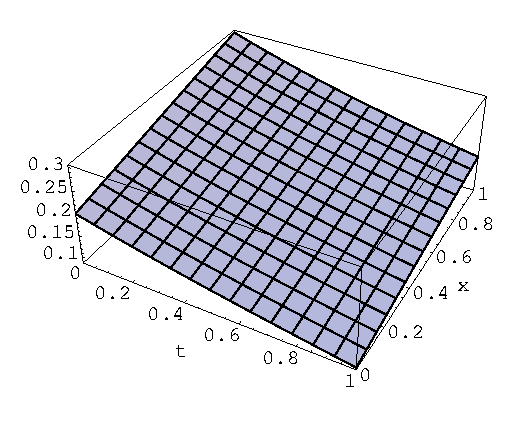
\includegraphics{graph1.eps}}}\hspace{5pt}
% \subfigure[A slightly shorter sub-caption.]{%
% \resizebox*{5cm}{!}{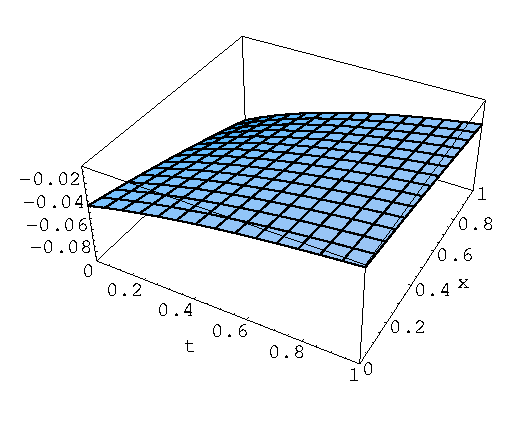
\includegraphics{graph2.eps}}}
% \caption{Example of a two-part figure with individual sub-captions
%  showing that captions are flush left and justified if greater
%  than one line of text.} \label{sample-figure}
% \end{figure}

% \begin{table}
% \tbl{Example of a table showing that its caption is as wide as
%  the table itself and justified.}
% {\begin{tabular}{lcccccc} \toprule
%  & \multicolumn{2}{l}{Type} \\ \cmidrule{2-7}
%  Class & One & Two & Three & Four & Five & Six \\ \midrule
%  Alpha\textsuperscript{a} & A1 & A2 & A3 & A4 & A5 & A6 \\
%  Beta & B2 & B2 & B3 & B4 & B5 & B6 \\
%  Gamma & C2 & C2 & C3 & C4 & C5 & C6 \\ \bottomrule
% \end{tabular}}
% \tabnote{\textsuperscript{a}This footnote shows how to include
%  footnotes to a table if required.}
% \label{sample-table}
% \end{table}


\bibliographystyle{tfcad}
\bibliography{linear_sensor_opti}
% \bibliography{interactcadsample}

\end{document}